
\documentclass[preprint,12pt]{elsarticle}
\makeatletter
\def\ps@pprintTitle{%
 \let\@oddhead\@empty
 \let\@evenhead\@empty
 \def\@oddfoot{\centerline{\thepage}}%
 \let\@evenfoot\@oddfoot}
\makeatother

\usepackage[spanish]{babel}
\usepackage{amssymb}
\usepackage{graphicx}
\usepackage{lineno}
\usepackage[utf8]{inputenc}
\usepackage{url}
\usepackage{natbib} 
\usepackage{amsmath} 
\usepackage{amssymb} 

\begin{document}
	\begin{frontmatter}
		\title{\huge Informe de Laboratorio Nro 07: Contenedor de Microsoft SQL Server}
		\author{Estrella Palacios, Katherine Lizbeth              	(2016056193)}	
		\address{Universidad Privada de Tacna}
		\address{Escuela Profesional de Ingeniería de Sistemas}
		\address{Tacna, Perú}
	\end{frontmatter}

%% INFORMACIÓN GENERAL -----------------------------------------------------------------------------------------------------------------------------------
\section{INFORMACIÓN GENERAL}
Objetivos:
	\begin{itemize}
		\item Crear un contenedor de la imagen de Microsoft SQL Server 
		\item Desplegar una BD usando un contenedor
	\end{itemize}
Equipos y programas utilizados:
Para el siguiente laboratorio requerimos de:
	\begin{itemize}
		\item PC con sistema operativo Windows 10
		\item Microsoft SQL Server Management Studio
		\item Docker Desktop
	\end{itemize}

%% MARCO TEORICO -----------------------------------------------------------------------------------------------------------------------------------
\section{MARCO TEÓRICO}
\subsection{\textbf{Historia}}
Salomon Hykes comenzó Docker comenzó como un proyecto interno dentro de dotCloud,empresa enfocada a PaaS (plataforma como servicio). Fué liberado como código abierto en marzode 2013.Con el lanzamiento de la versión 0.9 (en marzo de 2014) Docker dejó de utilizar LXC comoentorno de ejecución por defecto y lo reemplazó con su propia librería, libcontainer (escrita en Go),que se encarga de hablar directamente con el kernel.Actualmente es uno de los proyectos con más estrellas en GitHub, con miles debifurcaciones (forks) y miles de colaboradores.

\subsection{\textbf{Características}}
Las principales características de Docker son:


\begin{itemize}
\item \textbf{Portabilidad:} el contenedor Docker podemos desplegarlo en cualquier sistema, sin necesidad de volver a configurarlo o realizar las instalaciones necesarias para que la aplicación funcione, ya que todas las dependencias son empaquetadas con la aplicación en el contenedor.

\item \textbf{Ligereza:} los contenedores Docker sólo contienen lo que las diferencia del sistema operativo en el que se ejecutan, no se virtualiza un SO completo.

\item \textbf{Autosuficiencia:} un contenedor Docker no contiene todo un sistema operativo completo,sólo aquellas librerías, archivos y configuraciones necesarias para desplegar las funcionalidades que contenga.

\end{itemize}

\subsection{\textbf{Ventajas y Desventajas}}
Usar contenedores Docker permite a des arrolladores y administradores de sistemas probar aplicaciones o servicios en un entorno seguro e igual al de producción, reduciendo los tiempos de pruebas y adaptaciones entre los entornos de prueba y producción. Las principales ventajas de usar contenedores Docker son:

\begin{itemize}
\item Las instancias se inician en pocos segundos.
\item Son fácilmente replicables.
\item Es fácil de automatizar e integrar en entornos de integración continua.
\item Consumen menos recursos que las máquinas virtuales tradicionales.
\item Mayor rendimiento que la virtualización tradicional ya que corre directamente sobre el Kernel de la máquina en la que se aloja, evitando al hypervisor.
\item Ocupan mucho menos espacio.
\item Aisla las dependencias de una aplicación de las instaladas en el host.
\item Existe un gran repositorio de imágenes ya creadas sobre miles de aplicaciones, que además pueden modificarse libremente.

\end{itemize}

Por todo esto Docker ha entrado con mucha fuerza en el mundo del desarrollo, ya que permite desplegar las aplicaciones en el mismo entorno que tienen en producción o viceversa,permite desarrollarlas en el mismo entorno que tendrán en producción. Aunque también tiene algunas desventajas:

\begin{itemize}
\item Sólo puede usarse de forma nativa en entornos Unix con Kernel igual o superior a 3.8.
\item Sólo soporta arquitecturas de 64 bits.
\item Como es relativamente nuevo, puede haber errores de código entre versiones.

\end{itemize}

\subsection{\textbf{Arquitectura}}
Docker usa una arquitectura cliente-servidor. El cliente de Docker habla con el demonio de Docker que hace el trabajo de crear, correr y distribuir los contenedores. Ambos pueden ejecutarse en el mismo sistema, o se puede conectar un cliente a un demonio Docker remoto. El cliente Dockery el demonio se comunican vía sockets o a través de una RESTfull API. (imagen pagina oficial. \\ \\Explicamos un poco por orden la arquitectura o funcionamiento de Docker: 
\begin{itemize}
\item El cliente de Docker (Docker Client) es la principal interfaz de usuario para Docker. Él acepta comandos del usuario y se comunica con el demonio Docker.
\item El demonio Docker (Docker Engine) corre en una máquina anfitriona (host). El usuario no interactúa directamente con el demonio, en su lugar lo hace a través del cliente Docker.
\item El demonio Docker levanta los contenedores haciendo uso de las imágenes, que puedenestar en local o en el Docker Registry. 
\item Cada contenedor se crea a partir de una imagen y es un entorno aislado y seguro dónde seejecuta nuestra aplicación.
\end{itemize}

\begin{figure}[htb]
	\begin{center}
		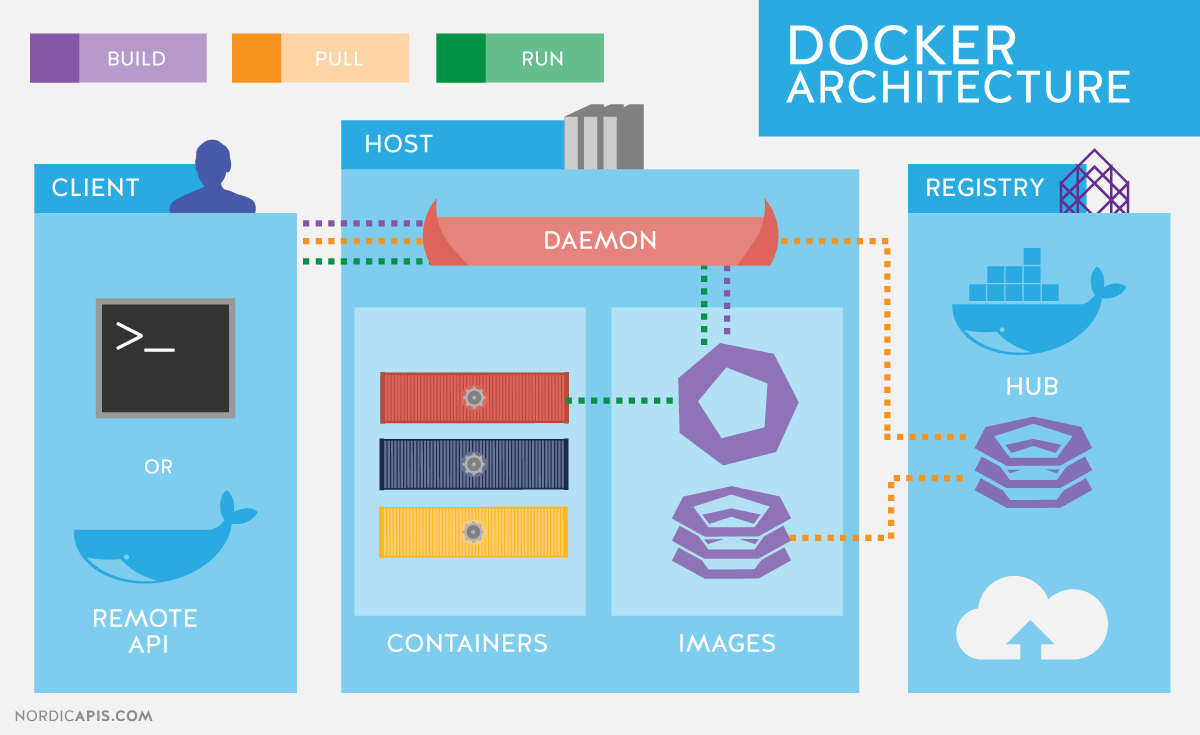
\includegraphics[width=13cm]{./IMAGENES/arquitectura}
	\end{center}
\end{figure}

\subsection{\textbf{Componentes}}
Según la documentación oficial, Docker tiene dos principales componentes:

\begin{itemize}
\item \textbf{Docker:} Plataforma open source de virtualización con contenedores.
\item \textbf{Docker Hub:} Plataforma de Software como servicio (SaaS, Software-as-a-Service) para compartir y administrar contenedores Docker.
\end{itemize}

\begin{figure}[htb]
	\begin{center}
		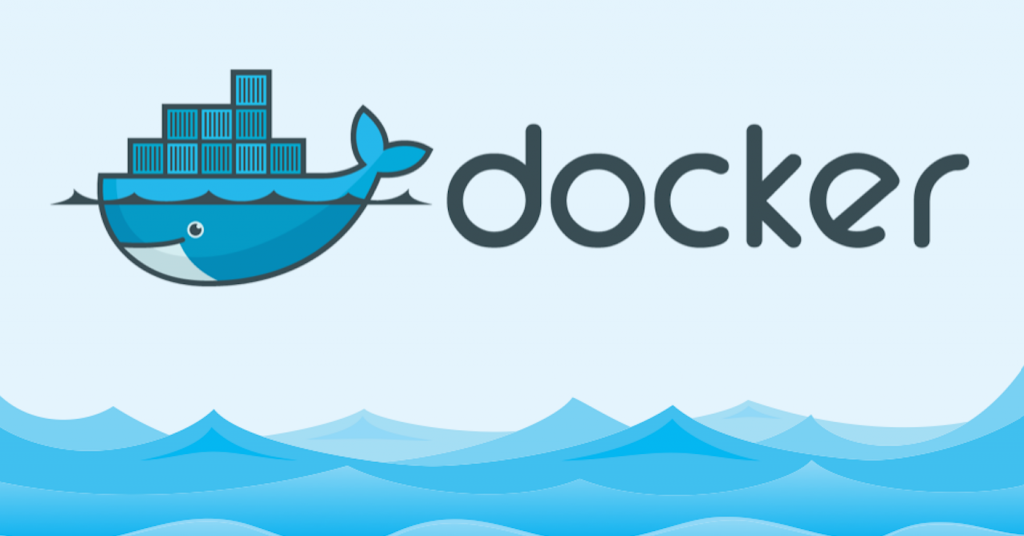
\includegraphics[width=9cm]{./IMAGENES/docker}
	\end{center}
\end{figure}

Pero también necesitamos conocer otros componentes y conceptos:

\begin{itemize}
\item \textbf{Docker Engine:} Es el demonio que se ejecuta dentro del sistema operativo (Linux) y que expone una API para la gestión de imágenes, contenedores, volúmenes o redes. 
\item \textbf{Docker Client:} Cualquier software o herramienta que hace uso de la API del demonio Docker, pero suele ser el comando docker, que es la herramienta de línea de comandos para gestionar Docker Engine.Éste cliente puede configurarse para hablar con un Docker local o remoto, lo que permite administrar nuestro entorno de desarrollo local como nuestros servidores de producción.
\item \textbf{Docker Images:} Son plantillas de sólo lectura que contienen el sistema operativo base (más adelante entraremos en profundidad) dónde correrá nuestra aplicación, además de las dependencias y software adicional instalado, necesario para que la aplicación funcione correctamente. Las plantillas son usadas por Docker Engine para crear los contenedores Docker.
\item \textbf{Docker Registries:} Los registros de Docker guardan las imágenes. Pueden ser repositorios públicos o privados.El registro público lo provee el Hub de Docker, que sirve tanto imágenes oficiales cómo las subidas por usuarios con sus propias aplicaciones y configuraciones.
\item \textbf{Docker Containers:} El contenedor de Docker aloja todo lo necesario para ejecutar un servicio o aplicación. Cada contenedor es creado de una imagen base y es una plataforma aislada.
\item \textbf{Docker Compose:} Es otro proyecto open source que permite definir aplicaciones multi-contenedor de una manera sencilla. Es una alternativa más cómoda al uso del comando docker run, para trabajar con aplicaciones con varios componentes.
\item \textbf{Docker Machine:} Es un proyecto open source para automatizar la creación de máquinas virtuales con Docker instalado, en entornos Mac, Windows o Linux, pudiendo administrar así un gran número de máquinas Docker.Incluye drivers para Virtualbox, que es la opción aconsejada para instalaciones de Docker en local, en vez de instalar Docker directamente en el host. 
\end{itemize}


%% PROCEDIMIENTO -----------------------------------------------------------------------------------------------------------------------------------
\section{PROCEDIMIENTO}
\textbf{Paso 1 : Iniciar Docker}
\begin{enumerate}[a)]
\item Iniciaremos con nuesytra cuenta docker en Docker Deskot.
\begin{figure}[htb]
	\begin{center}
		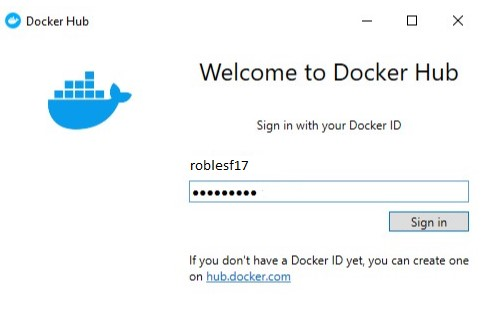
\includegraphics[width=8cm]{./IMAGENES/Docker01}
	\end{center}
\end{figure}
\item Debemos estar registrados para ingresar.
\item Ejecutamos PowerShell y agregamos el siguiente comando \textbf{docker version}.
\begin{figure}[htb]
	\begin{center}
		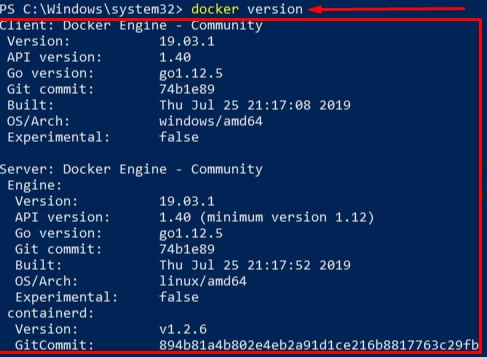
\includegraphics[width=6cm]{./IMAGENES/Docker02}
	\end{center}
\end{figure}


\textbf{Paso 2 : Crearemos un contenedor con Microsoft SQL Server para Linux}
\item Ejecutaremos el siguiente comando \textbf{docker search mssql} en PowerShell.
\begin{figure}[htb]
	\begin{center}
		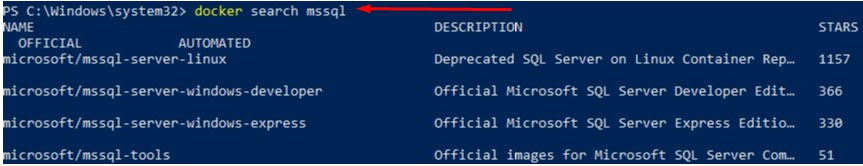
\includegraphics[width=11cm]{./IMAGENES/Docker03}
	\end{center}
\end{figure}
\item Ingraseremos nuestra cuenta en la página web Desktop Hub y buscaremos el repositorio \textbf{"microsoft/mssql-server-linux"}. 
\begin{figure}[htb]
	\begin{center}
		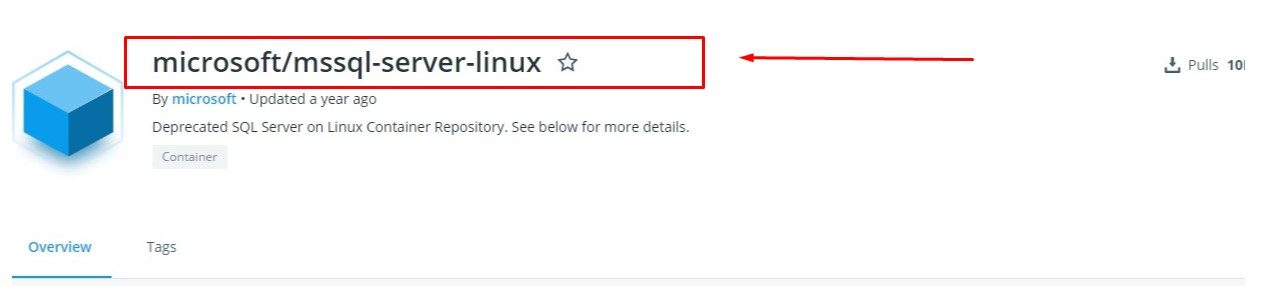
\includegraphics[width=9cm]{./IMAGENES/Docker04}
	\end{center}
\end{figure}
\item Copiando el comando en la aplicación PowerShell (docker pull microsoft/mssql-server-linux)
Se descargará la imagen del contenedor de Microsoft SQL Server en un servidor Linux como podemos ver en la imagen.
\begin{figure}[htb]
	\begin{center}
		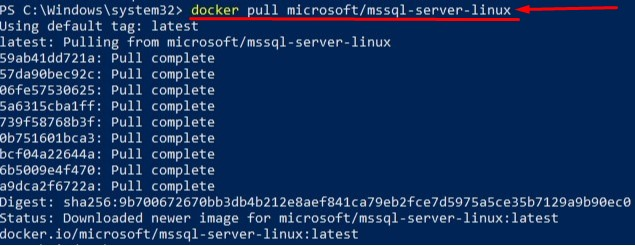
\includegraphics[width=11cm]{./IMAGENES/Docker05}
	\end{center}
\end{figure}


\item Verificaremos la imagen descargada con el siguiente comando \textbf{docker images}.
\begin{figure}[htb]
	\begin{center}
		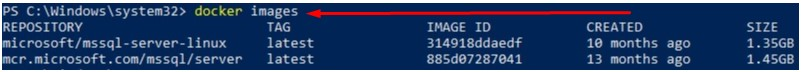
\includegraphics[width=14cm]{./IMAGENES/Docker06}
	\end{center}
\end{figure}

\item Iniciaremos el contenedor con el siguiente comando
\begin{figure}[htb]
	\begin{center}
		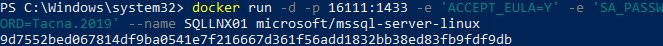
\includegraphics[width=14cm]{./IMAGENES/Docker07}
	\end{center}
\end{figure}

\item Nos devolcera el ID del contenedor.
\begin{center}
9d7552bed067814df9ba0541e7f216667d361f56add1832bb38ed83fb9fdf9db
\end{center}

\item Verificamos que el contenedor se está ejecutando correctamente con el siguiente comando docker ps. El resultado será similar al siguiente:
\begin{figure}[htb]
	\begin{center}
		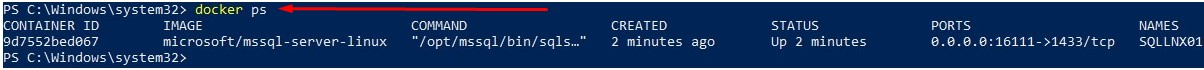
\includegraphics[width=14cm]{./IMAGENES/Docker08}
	\end{center}
\end{figure}

\item Abriremos el programa Microsoft SQL Server Management Studio 17 y conectamos con los siguientes datos: 
\begin{center}Nombre del servidor : 127.0.0.1,16111\end{center}
\begin{center} Inicio de sesión :sa\end{center}
\begin{center}Contraseña:Epis2019\end{center}
	\begin{figure}[htb]
		\begin{center}
		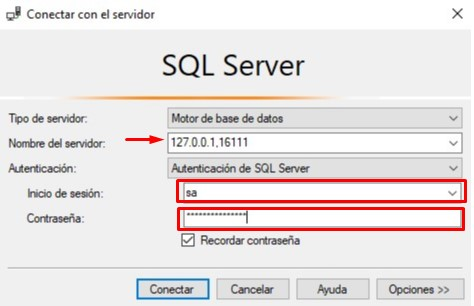
\includegraphics[width=6.5cm]{./IMAGENES/Docker13}
		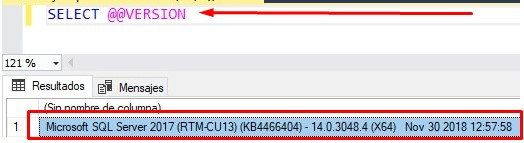
\includegraphics[width=6.5cm]{./IMAGENES/Docker11}
		\end{center}
	\end{figure}

\item Iniciaremos una consulta ingresando lo siguiente : 
\begin{center}SELECT @@VERSION\end{center}

\item En la aplicación PowerShell ejecutamos el siguiente comando:
\begin{center}docker rm -f SQLLNX01\end{center}
\item Verificamos la eliminación del contenedor con el siguiente comando:
\begin{center}docker ps\end{center}
\end{enumerate}

%% ANÁLISIS E INTERPRETACIÓN DE RESULTADOS -----------------------------------------------------------------------------------------------------------------------------------
\section{ANÁLISIS E INTERPRETACIÓN DE RESULTADOS}
\begin{enumerate}[a)]
\item Con el comando para iniciar con un contenedor podemos asignar los siguientes parámetros:
\begin{center} -p : 	Asignar el puerto.\end{center}
\begin{center}'sapassword' : Contraseña del Inicio de Sesion SQL, usuario sa.\end{center}
\begin{center} --name : Nombre del contenedor.\end{center}
\end{enumerate}


\section{CUESTIONARIO}

\begin{enumerate}[a)]
\item \textbf{¿Con qué comando(s) exportaría la imagen de Docker de Microsoft SQL Server a otra PC o servidor?}\newline
\\Exportar la Imagen de Docker de Microsoft SQL Server
"docker export (ID contenedor) >  Nombreimagen.tar"
\begin{center} docker 9d7552bed067814df9ba0541e7f216667d361f56add1832bb38ed83fb9fdf9db > SQL.tar \end{center}
\begin{figure}[htb]
	\begin{center}
		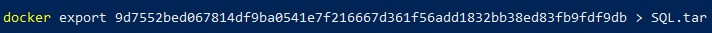
\includegraphics[width=14cm]{./IMAGENES/Docker17}
	\end{center}
\end{figure}
\item \textbf{¿Con qué comando(s) podría generar dos volúmenes para un contenedor para distribuir en un volumen el Archivo de Datos (.mdf) y en otro el Archivo Log (.ldf)?}\newline
\\CREATE DATABASE NAMEDATABASE ON \newline
( FILENAME = N'/var/opt/mssql/data2/NDATABASE.mdf' ),\newline
( FILENAME = N'/var/opt/mssql/data2/NDATABASElog.ldf' )\newline
FOR ATTACH\newline
GO\newline

\item \textbf{Genere un nuevo contenedor y cree la base de datos con las siguientes características.}\newline
\\Nombre : FINANCIERA \newline
Archivos:
\begin{itemize}
\item DATOS (mdf) : Tamaño Inicial : 50MB, Incremento: 10MB, Ilimitado
\item INDICES (ndf) Tamaño Inicial : 100MB, Incremento: 20MB, Maximo: 1GB
\item HISTORICO (ndf) Tamaño Inicial : 100MB, Incremento: 50MB, Ilimitado
\item LOG (ldf) Tamaño Inicial : 10MB, Incremento: 10MB, Ilimitado
\end{itemize}

\textbf{\\ ¿Cuál sería el script SQL que generaría esta base de datos?}
\begin{figure}[htb]
	\begin{center}
		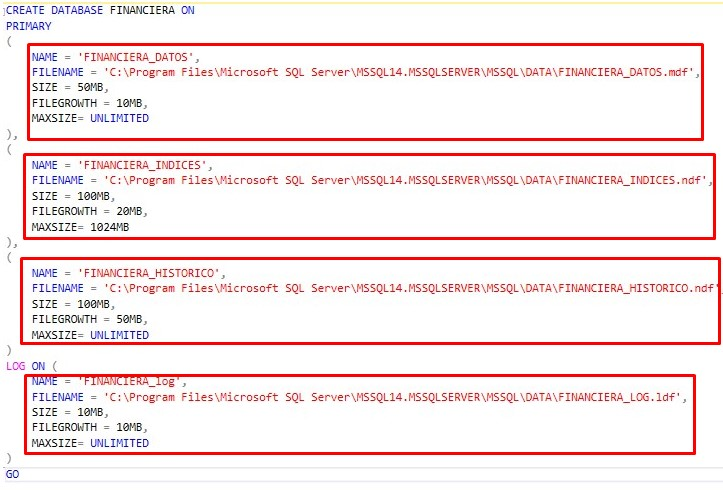
\includegraphics[width=9cm]{./IMAGENES/Docker14}
		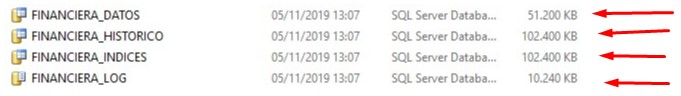
\includegraphics[width=9cm]{./IMAGENES/Docker15}
	\end{center}
\end{figure}
\end{enumerate}



\section{CONCLUSIONES}
Los contenedores de Docker nacen a partir de una imagen y en estos contenedores podemos solo ejecutar e instalar servicios, viene siendo como crear una maquina virtual a partir de una imagen (snapshot) pero muchísimo más ligera. 


\end{document}
